
\chapter{Linear PDEs: a structured grid example}
\label{chap:structured}

We start with the Poisson problem on a square because it is a straightforward PDE problem.  In solving this two-dimensional example we will learn how to use key parts of \PETSc: we will build a structured grid using a \PETSc \pDMDA, then assemble a \pMat in parallel based on this grid, and then solve in parallel using a \pKSP object.  We will generate a linear system comparable to, but more interesting than, ones we solved in Chapter \ref{chap:getstarted}.

\section{Poisson problem on a square domain}

Let $\mathcal{S}$ be the open unit square $(0,1)\times(0,1)$ with boundary $\partial\mathcal{S}$.  The following is our \emph{Poisson problem} for this Chapter;  see Figure \ref{fig:unitsquare}:
\begin{align}
- \grad^2 u &= f \quad \text{ on } \mathcal{S}, \label{poissonsquare} \\
u &= 0 \quad \text{ on } \partial \mathcal{S}. \label{poissonsquarebcs}
\end{align}
In \eqref{poissonsquare} the \emph{Laplacian} of $u(x,y)$ is
    $$\grad^2 u = \Div(\grad u) = \frac{\partial^2 u}{\partial x^2} + \frac{\partial^2 u}{\partial y^2}.$$

\begin{marginfigure}
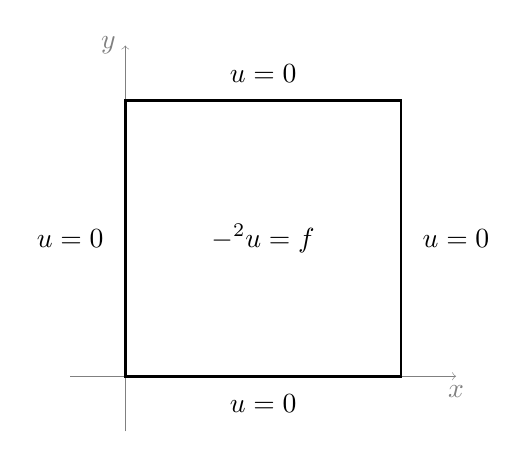
\begin{tikzpicture}[scale=3.5]
  \draw[->,gray,very thin] (-0.2,0.0) -- (1.2,0.0) node[below] {$x$};
  \draw[->,gray,very thin] (0.0,-0.2) -- (0.0,1.2) node[left] {$y$};
  \draw[line width=1.0pt] (0.0,0.0) -- (0.0,1.0) -- (1.0,1.0) -- (1.0,0.0) -- cycle;
  \node at (0.5,0.5) {$- \grad^2 u = f$};
  \node at (0.5,-0.1) {$u = 0$};
  \node at (0.5,1.1) {$u = 0$};
  \node at (-0.2,0.5) {$u = 0$};
  \node at (1.2,0.5) {$u = 0$};
\end{tikzpicture}
\caption{Our first goal is to solve the Poisson equation on the unit square $\mathcal{S}$, with homogeneous Dirichlet boundary conditions.}
\label{fig:unitsquare}
\end{marginfigure}

The Laplacian almost always appears in mathematical models through some sense of conservation of $u$, along with an assumption that the flux of $u$ is proportional to the gradient of $u$ \citep{Ockendonetal2003}.  The divergence ``$\Div$'' factor of the Laplacian arises from a connection between a flux integral over a closed surface and an integral over the interior of that surface, namely the divergence (Gauss-Green) theorem \citep[Appendix C]{Evans}.

The PDE \eqref{poissonsquare} itself is the \emph{Poisson equation}, and equation \eqref{poissonsquarebcs} represents \emph{homogeneous Dirichlet} boundary conditions.  Historically speaking, \eqref{poissonsquare} and \eqref{poissonsquarebcs} form the \emph{Dirichlet problem} if $f=0$ and the boundary conditions are given by some $g$ along $\partial S$, but we call all instances of the problem ``Poisson'' as we will consider various boundary conditions (Chapter \ref{chap:unstructured}) but always allow non-zero right-hand side $f$.  Of course, the problem must have proper types of boundary conditions, either Dirichlet ($u$ known) or Neumann (derivative of $u$ known), or the right combinations, if it is to determine a unique solution.  The Poisson problem may model the electrostatic potential, the equilibrium distribution from certain random walks, or various other other physical phenomena.

For example, in the context of heat conduction in solids Fourier's law says that the heat flux is $\bq = -k \grad u$, where $k$ is the conductivity.  Conservation of heat energy says $c\rho \partial u/\partial t = - \Div\bq + f$ if $f$ describes a heat source within the domain.  The coefficient ``$c\rho$'' parameterizes the ability of the material to hold heat by a gain in temperature \citep{Ockendonetal2003}.  At steady state these facts combine to give $0 = k \grad^2 u + f$ in the simple case where $k$ is constant.  Thus Poisson's equation \eqref{poissonsquare}.  Holding the temperature fixed at zero along the boundary, i.e.~\eqref{poissonsquarebcs}, completes the problem we will consider.  Holding the heat flux fixed along the boundary, i.e.~Neumann conditions, is just as common and often more physical.

With homogeneous Neumann boundary conditions, the Poisson equation $-\grad^2 u = f$ is not a well-posed problem because if $u$ is a solution then $v=u+C$ is also a solution for any constant $C$.  Without any boundary conditions, there are infinitely-many solutions to the Laplace equation $-\grad^2 w = 0$ on $\mathcal{S}$ (\emph{harmonic functions}), so the Poisson equation is far from well-posed because if $u$ solves $-\grad^2 u = f$ then so does $v=u+w$.  However, with the Dirichlet boundary conditions in \eqref{poissonsquarebcs}, the solution is unique if it exists.\sidenote{See Theorem 5 in section 2.2 in \citep{Evans} or subsection 5.2.1 of \citep{Ockendonetal2003}.}

In this Chapter we will also require that $f(x,y)$ be continuous and bounded on $\mathcal{S}$, so that we can compute its pointwise values.  With our homogeneous Dirichlet boundary conditions, and this assumption on $f$, standard theory says that $u(x,y)$ exists and is continuous on the closed square $\bar{\mathcal{S}}$ \citep[Theorem 6 in section 5.6]{Evans}.\sidenote{A classical approach to showing existence starts by solving problem \eqref{poissonsquare} by Fourier series.  If $f$ is square-integrable then the coefficients $\hat f$ are square-integrable (Parseval's equality).  Because the Laplacian is elliptic and second-order, the coefficients $\hat u$ are square-integrable even when multiplied by the frequency squared.  By Cauchy-Schwarz, the Fourier series for $u$ is the limit of a sequence of continuous functions on $\overline{\mathcal{S}}$ which converge uniformly, so $u\in C^0(\overline{\mathcal{S}})$.}  Thus there is no ambiguity in the boundary condition ``$u=0$ on $\partial \mathcal{S}$'' and we can sensibly evaluate pointwise errors if we have an exact solution. 


\section{Building a structured grid}

Because \eqref{poissonsquare} and \eqref{poissonsquarebcs} for a linear problem, finite-dimensional approximations of it are simply linear systems.  The approximation in this Chapter comes from applying a \emph{finite difference} (FD) method as a way to generate the linear system.  In Chapter \ref{chap:unstructured} we will apply a finite element approach instead.

To start our FD method we put a \emph{structured grid} of $MN$ points on the unit square, as in Figure \ref{fig:unitsquaregrid}, with spacing $h_x=1/(M-1)$ and $h_y=1/(N-1)$ in the two directions.  The grid coordinates are $x_i = i\, h_x$ for $i = 0,1,\dots,M-1$ and $y_j = j\, h_y$ and $j=0,1,\dots,N-1$.  The construction of such a two-dimensional (2D) grid, and distributing it across processors, will form our first new ideas from \PETSc, beyond the basics in Chapter \ref{chap:getstarted}.

\begin{marginfigure}
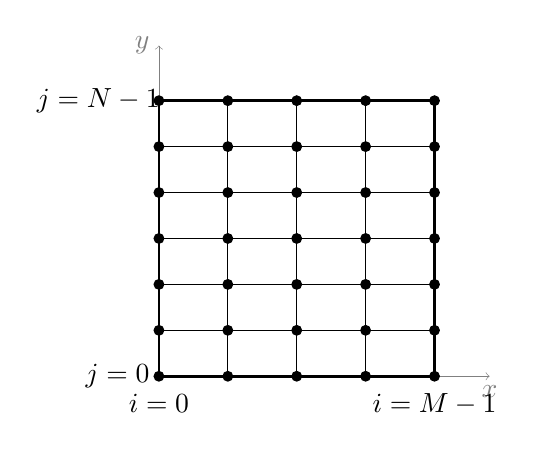
\begin{tikzpicture}[scale=3.5]
  \draw[->,gray,very thin] (0.0,0.0) -- (1.2,0.0) node[below] {$x$};
  \draw[->,gray,very thin] (0.0,0.0) -- (0.0,1.2) node[left] {$y$};
  \draw[line width=1.0pt] (0.0,0.0) -- (0.0,1.0) -- (1.0,1.0) -- (1.0,0.0) -- cycle;
  \node at (0.0,-0.1) {$i=0$};
  \node at (1.0,-0.1) {$i=M-1$};
  \node at (-0.15,0.0) {$j=0$};
  \node at (-0.22,1.0) {$j=N-1$};
  \pgfmathsetmacro\fourth{1.0/4.0}
  \pgfmathsetmacro\sixth{1.0/6.0}
  \draw[xstep=\fourth,ystep=\sixth,black,thin] (0.0,0.0) grid (1.0,1.0);
  \foreach \x in {0,...,4} {
    \foreach \y in {0,...,6} {
        \filldraw (\x * \fourth,\y * \sixth) circle (0.5pt);
    }
  }
\end{tikzpicture}
\caption{A grid on the unit square $\mathcal{S}$, with $M=5$ and $N=7$.}
\label{fig:unitsquaregrid}
\end{marginfigure}

Consider the lines of code in Figure \ref{code:dmdacreatetwod}, an extract from \texttt{c2poisson.c} later in this Chapter.  These lines create a \PETSc \pDM object for a grid like Figure \ref{fig:unitsquaregrid}.  A \pDM is an abstract type for describing the topology (connectedness) of a grid, \emph{and} the way it is distributed across \MPI processes, \emph{and} the way each process can access data from its neighboring processes.  The specific case in Figure \ref{code:dmdacreatetwod} creates a ``\pDMDA'', which is the subclass of \pDM s which are structured grids.  (``\pDM'' might stand for ``distributed mesh,'' and ``\texttt{DA}'' for ``distributed array''.)

\cinputraw{dmdacreate2d.frag}{extract from c2poisson.c}{An example of creating a 2D \pDMDA.  See Figures \ref{code:ctwopoissoncreate} and \ref{code:ctwopoissonsolve} for the rest of this code.}{}{//START}{//STOP}{code:dmdacreatetwod}

If we do
\begin{cline}
$ make c2poisson
$ ./c2poisson -da_grid_x 5 -da_grid_y 7
\end{cline}
then the structured grid shown in Figure \ref{fig:unitsquaregrid} is created.  In this case all points of the grid are ``owned'' by the single process invoked when we ran \texttt{c2poisson} (i.e.~without \MPI).

\begin{marginfigure}
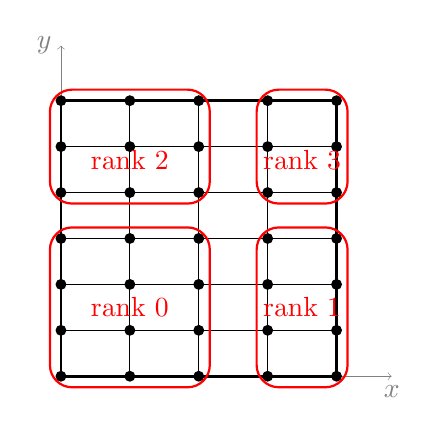
\begin{tikzpicture}[scale=3.5]
  \draw[->,gray,very thin] (0.0,0.0) -- (1.2,0.0) node[below] {$x$};
  \draw[->,gray,very thin] (0.0,0.0) -- (0.0,1.2) node[left] {$y$};
  \draw[line width=1.0pt] (0.0,0.0) -- (0.0,1.0) -- (1.0,1.0) -- (1.0,0.0) -- cycle;
  \pgfmathsetmacro\fourth{1.0/4.0}
  \pgfmathsetmacro\sixth{1.0/6.0}
  \draw[xstep=\fourth,ystep=\sixth,black,thin] (0.0,0.0) grid (1.0,1.0);
  \foreach \x in {0,...,4} {
    \foreach \y in {0,...,6} {
        \filldraw (\x * \fourth,\y * \sixth) circle (0.5pt);
    }
  }
  \pgfmathsetmacro\dd{0.04}
  \pgfmathsetmacro\od{1.04}
  \pgfmathsetmacro\xap{2*\fourth + 0.04}
  \pgfmathsetmacro\xbm{3*\fourth - 0.04}
  \pgfmathsetmacro\yap{3*\sixth + 0.04}
  \pgfmathsetmacro\ybm{4*\sixth - 0.04}
  \pgfmathsetmacro\xamid{1*\fourth}
  \pgfmathsetmacro\xbmid{3.5*\fourth}
  \pgfmathsetmacro\yamid{1.5*\sixth}
  \pgfmathsetmacro\ybmid{4.7*\sixth}
  \draw[thick,rounded corners=8pt,color=red]
    (-\dd,-\dd) -- (-\dd,\yap) -- (\xap,\yap) -- (\xap,-\dd) -- cycle;
  \node[color=red] at (\xamid,\yamid) {rank $0$};
  \draw[thick,rounded corners=8pt,color=red]
    (\xbm,-\dd) -- (\od,-\dd) -- (\od,\yap) -- (\xbm,\yap) -- cycle;
  \node[color=red] at (\xbmid,\yamid) {rank $1$};
  \draw[thick,rounded corners=8pt,color=red]
    (-\dd,\ybm) -- (\xap,\ybm) -- (\xap,\od) -- (-\dd,\od) -- cycle;
  \node[color=red] at (\xamid,\ybmid) {rank $2$};
  \draw[thick,rounded corners=8pt,color=red]
    (\xbm,\ybm) -- (\od,\ybm) -- (\od,\od) -- (\xbm,\od) -- cycle;
  \node[color=red] at (\xbmid,\ybmid) {rank $3$};
\end{tikzpicture}
\caption{The same grid as in Figure \ref{fig:unitsquaregrid}, distributed across four \MPI processes (i.e.~with \texttt{rank} $\in \{0,1,2,3\}$) automatically by \texttt{DMDACreate2d()}.}
\label{fig:unitsquaregridparallel}
\end{marginfigure}

However, if we run with multiple \MPI processes by
\begin{cline}
$ mpiexec -n N ./c2poisson -da_grid_x Mx -da_grid_y My
\end{cline}
%$
then \PETSc does the best it can to balance the load of \texttt{Mx}$\cdot$\texttt{My} grid points among \texttt{N} processes, with the restriction that each \MPI process owns a rectangular subgrid.  For example, if we do
\begin{cline}
$ mpiexec -n 4 ./c2poisson -da_grid_x 5 -da_grid_y 7
\end{cline}
%$
then the distributed structured grid shown in Figure \ref{fig:unitsquaregridparallel} will be created.  Neither \texttt{Mx}$=5$ nor \texttt{My}$=7$ is divisible by two, but \PETSc distributes the four ranks across the \texttt{Mx}$\cdot$\texttt{My}$=35$ nodes (grid points) relatively uniformly: the rank $0$ process owns 12 grid points and the rank $3$ process owns 6, while the other ranks are in between.  In this case the load is only balanced to within a factor of two, but larger grids can be better load-balanced.

\begin{marginfigure}
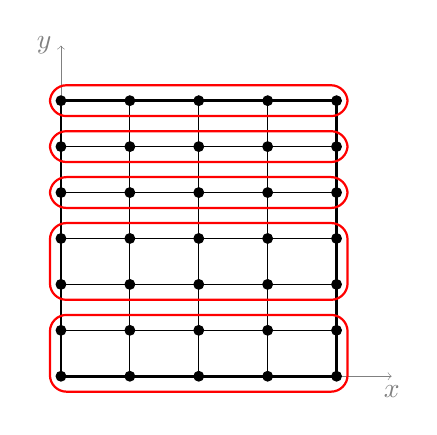
\begin{tikzpicture}[scale=3.5]
  \draw[->,gray,very thin] (0.0,0.0) -- (1.2,0.0) node[below] {$x$};
  \draw[->,gray,very thin] (0.0,0.0) -- (0.0,1.2) node[left] {$y$};
  \draw[line width=1.0pt] (0.0,0.0) -- (0.0,1.0) -- (1.0,1.0) -- (1.0,0.0) -- cycle;
  \pgfmathsetmacro\fourth{1.0/4.0}
  \pgfmathsetmacro\sixth{1.0/6.0}
  \draw[xstep=\fourth,ystep=\sixth,black,thin] (0.0,0.0) grid (1.0,1.0);
  \foreach \x in {0,...,4} {
    \foreach \y in {0,...,6} {
        \filldraw (\x * \fourth,\y * \sixth) circle (0.5pt);
    }
  }
  \pgfmathsetmacro\dd{0.04}
  \pgfmathsetmacro\od{1.04}
  \foreach \y in {0,2} {
    \pgfmathsetmacro\yup{\y * \sixth - 1.4 * \dd}  % less than 1.7 generates flaw?
    \pgfmathsetmacro\ydn{(\y + 1) * \sixth + 1.4 * \dd}
    \draw[thick,rounded corners=6pt,color=red]
      (-\dd,\ydn) -- (\od,\ydn) -- (\od,\yup) -- (-\dd,\yup) -- cycle;
  }
  \foreach \y in {4,5,6} {
    \pgfmathsetmacro\yup{\y * \sixth - 1.4 * \dd}  % less than 1.7 generates flaw?
    \pgfmathsetmacro\ydn{\y * \sixth + 1.4 * \dd}
    \draw[thick,rounded corners=6pt,color=red]
      (-\dd,\ydn) -- (\od,\ydn) -- (\od,\yup) -- (-\dd,\yup) -- cycle;
  }
\end{tikzpicture}
\caption{Processor domains are far from square if the number of \MPI processes is prime.}
\label{fig:unitsquaregridprime}
\end{marginfigure}

The observant reader has already noted that if the total number of processes \texttt{N}, in ``\texttt{mpiexec -n N},'' is prime then we get not-at-all-square processor domains.  For instance, the ``bad'' result from running
\begin{cline}
$ mpiexec -n 5 ./c2poisson -da_grid_x 5 -da_grid_y 7
\end{cline}
%$
is shown in Figure \ref{fig:unitsquaregridprime}.  Each process' portion of the grid has large perimeter-to-area ratio so that communication between processes will be large compared to the computation on each process.

\begin{marginfigure}
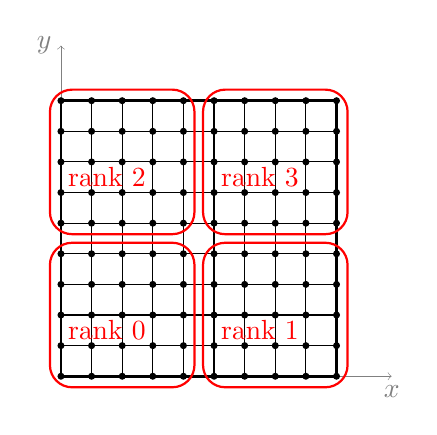
\begin{tikzpicture}[scale=3.5]
  \draw[->,gray,very thin] (0.0,0.0) -- (1.2,0.0) node[below] {$x$};
  \draw[->,gray,very thin] (0.0,0.0) -- (0.0,1.2) node[left] {$y$};
  \draw[line width=1.0pt] (0.0,0.0) -- (0.0,1.0) -- (1.0,1.0) -- (1.0,0.0) -- cycle;
  \pgfmathsetmacro\ninth{1.0/9.0}
  \draw[xstep=\ninth,ystep=\ninth,black,thin] (0.0,0.0) grid (1.0,1.0);
  \foreach \x in {0,...,9} {
    \foreach \y in {0,...,9} {
        \filldraw (\x * \ninth,\y * \ninth) circle (0.3pt);
    }
  }
  \pgfmathsetmacro\dd{0.04}
  \pgfmathsetmacro\od{1.04}
  \pgfmathsetmacro\ap{4*\ninth + 0.04}
  \pgfmathsetmacro\bm{5*\ninth - 0.04}
  \pgfmathsetmacro\amid{1.5*\ninth}
  \pgfmathsetmacro\bmid{6.5*\ninth}
  \draw[thick,rounded corners=8pt,color=red]
    (-\dd,-\dd) -- (-\dd,\ap) -- (\ap,\ap) -- (\ap,-\dd) -- cycle;
  \node[color=red] at (\amid,\amid) {rank $0$};
  \draw[thick,rounded corners=8pt,color=red]
    (\bm,-\dd) -- (\od,-\dd) -- (\od,\ap) -- (\bm,\ap) -- cycle;
  \node[color=red] at (\bmid,\amid) {rank $1$};
  \draw[thick,rounded corners=8pt,color=red]
    (-\dd,\bm) -- (\ap,\bm) -- (\ap,\od) -- (-\dd,\od) -- cycle;
  \node[color=red] at (\amid,\bmid) {rank $2$};
  \draw[thick,rounded corners=8pt,color=red]
    (\bm,\bm) -- (\od,\bm) -- (\od,\od) -- (\bm,\od) -- cycle;
  \node[color=red] at (\bmid,\bmid) {rank $3$};
\end{tikzpicture}
\caption{A well-balanced, compact-domain distribution of a $M=10$ by $N=10$ grid across four \MPI processes, created by \texttt{DMDACreate2d()}.}
\label{fig:unitsquaregrideight}
\end{marginfigure}

Though these defaults can be overridden by runtime options \texttt{-da\_grid\_x} and \texttt{-da\_grid\_y}, the fifth and sixth arguments ``\texttt{-10}'' of \texttt{DMDACreate2d()} in Figure \ref{code:dmdacreatetwod} are used to set default dimensions $M=10$ and $N=10$.  Thus
\begin{cline}
$ mpiexec -n 4 ./c2poisson
\end{cline}
%$
distributes a $10\times 10$ grid among four processes as in Figure \ref{fig:unitsquaregrideight}, with each rank owning a square subgrid of 25 nodes.

\PETSc itself can show the parallel layout by option \texttt{-dm\_view}.  The alternative form \texttt{-dm\_view draw -draw\_pause 2}, or similar, shows the grid graphically using X windows.

To explain the other options to \texttt{DMDACreate2d()} we quote the \PETSc manual pages description:

\begin{code}
DMDACreate2d(MPI_Comm comm, DMBoundaryType bx, DMBoundaryType by,
  DMDAStencilType stype, PetscInt M, PetscInt N, PetscInt m, PetscInt n,
  PetscInt dof, PetscInt s, const PetscInt lx[], const PetscInt ly[],
  DM *da)
\end{code}
where
\small
\begin{itemize}[align=left]
\item[\texttt{comm}]   MPI communicator \\
\item[\texttt{bx,by}]  type of ghost nodes the array have; use one of \texttt{DM\_BOUNDARY\_NONE, DM\_BOUNDARY\_GHOSTED, DM\_BOUNDARY\_PERIODIC} \\
\item[\texttt{stype}] stencil type; use either \texttt{DMDA\_STENCIL\_BOX} or \texttt{DMDA\_STENCIL\_STAR} \\
\item[\texttt{M,N}]	   global dimension in each direction of the array; use \texttt{-M} and or \texttt{-N} to indicate that it may be set to a different value from the command line with \texttt{-da\_grid\_x <M> -da\_grid\_y <N>} \\
\item[\texttt{m,n}]   corresponding number of processors in each dimension (or \texttt{PETSC\_DECIDE} to have calculated) \\
\item[\texttt{dof}]     number of degrees of freedom per node \\
\item[\texttt{s}]       stencil width \\
\item[\texttt{lx,ly}]  arrays containing the number of nodes in each cell along the x and y coordinates, or \texttt{NULL}; if non-null, these must be of length as m and n, and the corresponding m and n cannot be \texttt{PETSC\_DECIDE}; the sum of the \texttt{lx[]} entries must be M, and the sum of the \texttt{ly[]} entries must be N \\
\item[\texttt{da}]      output: the resulting distributed array object 
\end{itemize}
\normalsize

In Figure \ref{code:dmdacreatetwod}, the second and third arguments are \texttt{DM\_BOUNDARY\_NONE} because our Dirichlet boundary conditions do not need communication to the next process' domain, nor periodic wrapping.  In the fourth argument we use \texttt{DMDA\_STENCIL\_STAR} because only cardinal neighbors of a grid point are used when forming the matrix; we picture the ``stencil'' below.  The two \texttt{PETSC\_DECIDE} arguments which follow tell \PETSc to distribute the grid over \MPI processes according to the size of (number of processes in) the \MPI communicator, and using \PETSc internal logic as illustrated above.  The next two arguments, in the ninth and tenth positions, say that our PDE is scalar (\texttt{dof}$=1$) and that the FD method only needs one neighbor in each \texttt{STENCIL\_STAR} direction (\texttt{s}$=1$).  The next two arguments after that are \texttt{NULL} because we are \emph{not} telling \PETSc any details about how to distribute processes over the grid; it \texttt{DECIDE}s for itself.  Finally, the \pDMDA object is created as an output (i.e.~pass-by-reference).

The call to \texttt{DMDASetUniformCoordinates()} in Figure \ref{code:dmdacreatetwod} sets the domain to be $[0,1]\times[0,1]$ in the sense that the \pDM object knows the spacing and locations of the grid points.  The last two arguments are ignored in this case; they would set limits on the third dimension if \texttt{da} were created with \texttt{DMDACreate3d()}.

\medskip
\begin{figure}
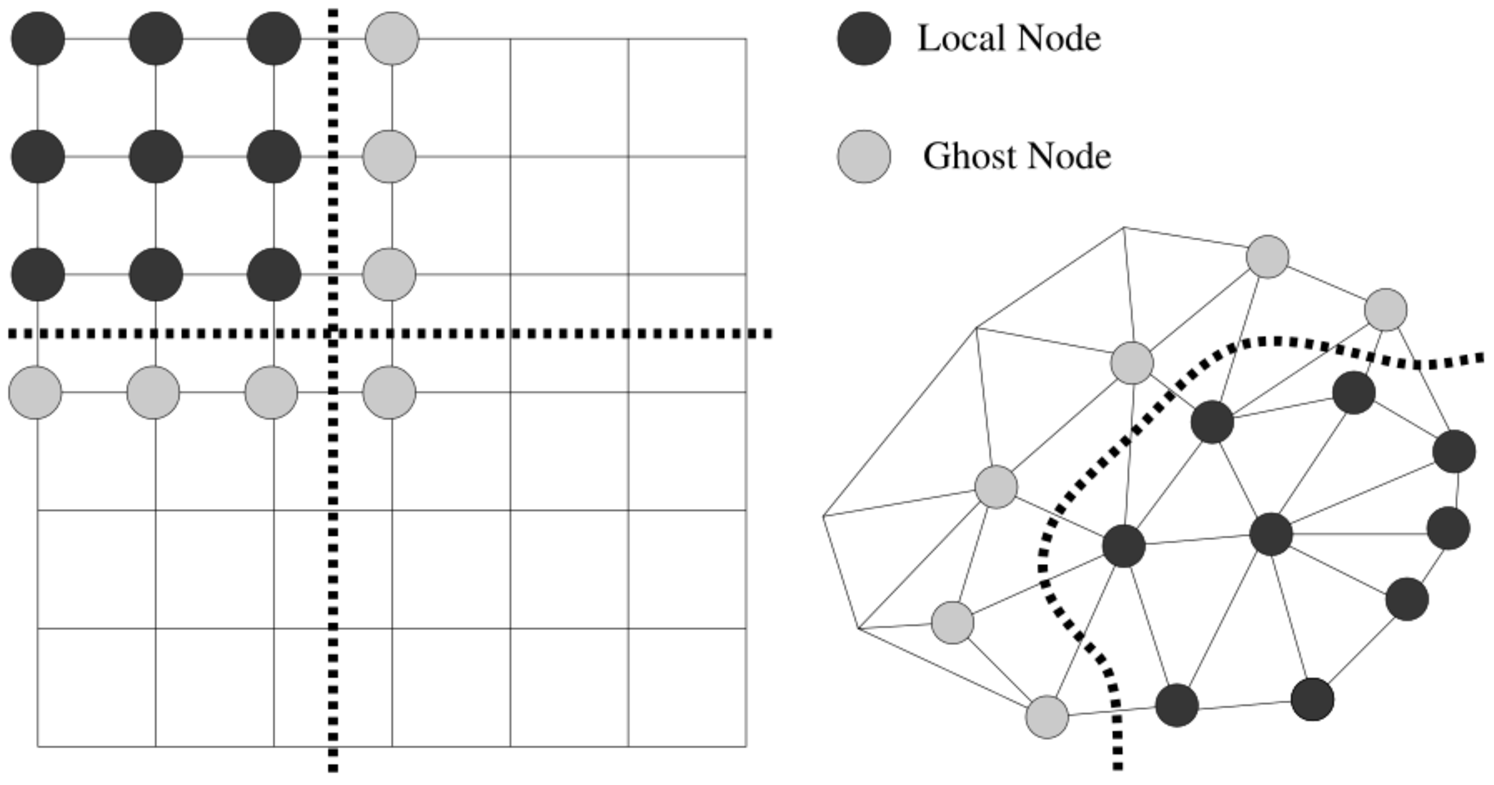
\includegraphics[width=\textwidth]{petscghostvalues}
\caption{\PETSc's parallel decomposition of structured (left) and unstructured (right) grids, showing owned (``local'') and accessible (``ghost'') nodes for one process.}
\label{fig:petscghostvalues}
\end{figure}

The standard \PETSc view of what \pDM s ``look like'' is in Figure \ref{fig:petscghostvalues}.  The code in Figure \ref{code:dmdacreatetwod} generates something like the left figure, namely a structured-grid \pDM, though the one shown in Figure \ref{fig:petscghostvalues} has \texttt{DMDA\_STENCIL\_BOX} stencil type, unlike ours.  On the right is an unstructured grid, of the type created in Chapter \ref{chap:unstructured} for the finite element method.  In both cases the Figure shows the nodes owned by a given process (red ``local'' nodes) and those other nodes that are accessible by the local process (blue ``ghost'' nodes).  We will see such local/ghost node types in all examples in this book.  We will return to them again in future examples.


\section{Finite difference method}

Recall we were trying to approximate PDE problem \eqref{poissonsquare} and \eqref{poissonsquarebcs}, not just build a grid!  The following finite difference method will allow us to take the next \PETSc step, which is to create and assemble \pVecs and a \pMat for the linear system corresponding to the PDE.

By a well-known Taylor's theorem argument \citep{MortonMayers}, for any function $F(x)$ which is sufficiently smooth we have
\begin{equation}
   F''(x) = \frac{F(x+h) - 2 F(x) + F(x-h)}{h^2} + O(h^2)  \label{secondderivativeFD}
\end{equation}
as $h$ goes to zero.  This formula, applied to partial derivatives, will approximate the Laplacian in equation \eqref{poissonsquare}.

Let $U_{i,j}$ be the gridded approximation to the value $u(x_i,y_j)$ of the exact solution $u(x,y)$ at a grid point,\sidenote{This is an important sentence!  We compute values $U_{i,j}$ from the finite difference equations.  We generally \emph{don't know} the values $u(x_i,y_j)$.  We do, however, want the former to be close to the latter.} and also denote $f_{i,j} = f(x_i,y_j)$.  From \eqref{secondderivativeFD} we have this FD approximation to equation \eqref{poissonsquare}:
\begin{equation}
- \frac{U_{i+1,j} - 2 U_{i,j} + U_{i-1,j}}{h_x^2} - \frac{U_{i,j+1} - 2 U_{i,j} + U_{i,j-1}}{h_y^2} = f_{i,j}. \label{poissonsquareFDearly}
\end{equation}
Equation \eqref{poissonsquareFDearly} applies at all of the interior points where $1 \le i \le M-2$ and $1 \le j \le N-2$.  The boundary conditions \eqref{poissonsquarebcs} become
\begin{equation}
U_{0,j} = 0, \quad U_{M-1,j} = 0, \quad U_{i,0} = 0, \quad U_{i,N-1} = 0, \label{poissonsquareFDbcs}
\end{equation}
for all $i,j$.

At grid location $(x_i,y_j)$, equation \eqref{poissonsquareFDearly} relates the unknown $U_{i,j}$ to its four cardinal neighbors $U_{i+1,j}$, $U_{i-1,j}$, $U_{i,j+1}$, and $U_{i,j-1}$.  This pattern is a \emph{stencil}, in particular a ``star'' stencil, as shown in Figure \ref{fig:unitsquaregridstencil}.  (A ``box'' stencil would additionally involve the four diagonal neighbors.  In 2D, a star stencil relates five unknowns, while a box stencil relates nine unknowns.)

We will treat all values $U_{i,j}$ on the grid, whether on the boundary or in the interior, as unknowns, so we have $K=MN$ unknowns.  Equations \eqref{poissonsquareFDearly} and \eqref{poissonsquareFDbcs} form a linear system of $K$ equations,
\begin{equation}
A \bu = \bb, \label{poissonlinearsystem}
\end{equation}
where $A$ is a $K\times K$ matrix and $\bu,\bb$ are $K\times 1$ column vectors.

\begin{marginfigure}
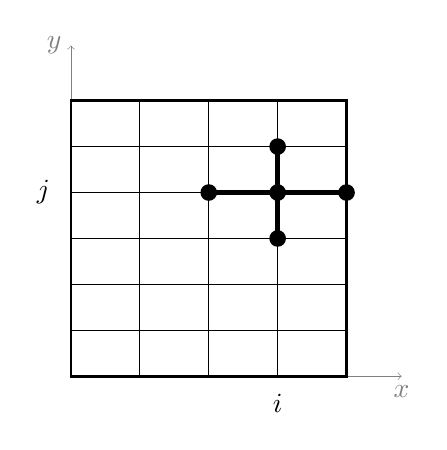
\begin{tikzpicture}[scale=3.5]
  \draw[->,gray,very thin] (0.0,0.0) -- (1.2,0.0) node[below] {$x$};
  \draw[->,gray,very thin] (0.0,0.0) -- (0.0,1.2) node[left] {$y$};
  \draw[line width=1.0pt] (0.0,0.0) -- (0.0,1.0) -- (1.0,1.0) -- (1.0,0.0) -- cycle;
  \node at (0.75,-0.1) {$i$};
  \node at (-0.1,0.666667) {$j$};
  \filldraw (0.50,0.666667) circle (0.8pt);
  \filldraw (0.75,0.666667) circle (0.8pt);
  \filldraw (1.00,0.666667) circle (0.8pt);
  \filldraw (0.75,0.5) circle (0.8pt);
  \filldraw (0.75,0.833333) circle (0.8pt);
  \draw[line width=2.0pt] (0.50,0.666667) -- (1.00,0.666667);
  \draw[line width=2.0pt] (0.75,0.5)  -- (0.75,0.833333);
  \draw[xstep=0.25,ystep=0.166667,black,thin] (0.0,0.0) grid (1.0,1.0);
\end{tikzpicture}
\caption{This ``star'' stencil simply illustrates the adjacency pattern in FD scheme \eqref{poissonsquareFDearly}.}
\label{fig:unitsquaregridstencil}
\end{marginfigure}

However, to show linear system \eqref{poissonlinearsystem} in traditional form we must globally-order the unknowns.  Such an ordering is implemented inside a \PETSc \pDMDA, but it is hidden so it can often be ignored.  While our code (\texttt{c2poisson.c} below) will only use the grid-wise coordinates $(i,j)$, we must be explicit about the ordering here for the purpose of displaying the system in matrix-vector form.  The ability to assemble \pMats and \pVecs with $(i,j)$-type indexing is one reason structured-grid codes using \pDMDA can be quite short.

The ordering used in a one-process (serial) run by a 2D \pDMDA is shown in Figure \ref{fig:unitsquaregridordering}.  On an $M$ by $N$ grid one could write it as
\begin{equation}
    U_k = U_{i,j} \quad \text{ where } \quad k = j\,M + i \label{orderingfd}
\end{equation}
for $i=0,1,\dots,M-1$ and $j=0,1,\dots,N-1$, so $k=0,1,\dots,MN-1$.  In fact we let \PETSc do such index transformations inside the \pDMDA implementation.

\begin{marginfigure}
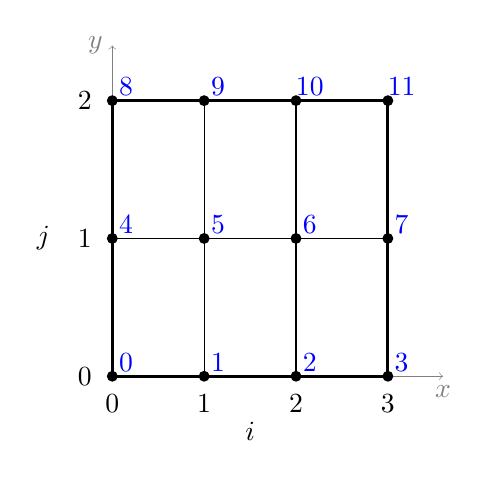
\begin{tikzpicture}[scale=3.5]
  \draw[->,gray,very thin] (0.0,0.0) -- (1.2,0.0) node[below] {$x$};
  \draw[->,gray,very thin] (0.0,0.0) -- (0.0,1.2) node[left] {$y$};
  \draw[line width=1.0pt] (0.0,0.0) -- (0.0,1.0) -- (1.0,1.0) -- (1.0,0.0) -- cycle;
  \pgfmathsetmacro\third{1.0/3.0}
  \pgfmathsetmacro\half{1.0/2.0}
  \node at (0.0,-0.1) {$0$};
  \node at (\third,-0.1) {$1$};
  \node at (\half,-0.2) {$i$};
  \node at (2*\third,-0.1) {$2$};
  \node at (1.0,-0.1) {$3$};
  \node at (-0.1,0.0) {$0$};
  \node at (-0.1,0.5) {$1$};
  \node at (-0.25,0.5) {$j$};
  \node at (-0.1,1.0) {$2$};
  \draw[xstep=\third,ystep=\half,black,thin] (0.0,0.0) grid (1.0,1.0);
  \pgfmathsetmacro\dd{0.05}
  \foreach \y in {0,1,2}
    \foreach \x in {0,1,2,3} {
      \pgfmathsetmacro\k{4*\y+\x}
      \draw[color=blue] (\x*\third+\dd,\y*\half+\dd) node{\pgfmathprintnumber[fixed]{\k}};
      \filldraw (\x * \third,\y * \half) circle (0.5pt);
    }
\end{tikzpicture}
\caption{Ordering of unknowns \eqref{orderingfd} on a $M=4$ and $N=3$ grid.  Index $k$ from \eqref{orderingfd} is shown in {\color{blue} blue}.}
\label{fig:unitsquaregridordering}
\end{marginfigure}

\medskip\noindent\hrulefill
\begin{example} In the $M=4$ and $N=3$ case (Figure \ref{fig:unitsquaregridordering}) we have grid spacing $h_x=1/3$ and $h_y=1/2$.  Only the $k=5$ and $k=6$ equations are not boundary conditions \eqref{poissonsquareFDbcs}.  The linear system \eqref{poissonlinearsystem} is
\setcounter{MaxMatrixCols}{20}
\begin{equation*}
\begin{bmatrix}
1 &  &  &  &  &  &  &  &  &  &  &  \\
  & 1&  &  &  &  &  &  &  &  &  &  \\
  &  & 1&  &  &  &  &  &  &  &  &  \\
  &  &  & 1&  &  &  &  &  &  &  &  \\
  &  &  &  & 1&  &  &  &  &  &  &  \\
  & c&  &  & b& a& b&  &  & c&  &  \\
  &  & c&  &  & b& a& b&  &  & c&  \\
  &  &  &  &  &  &  & 1&  &  &  &  \\
  &  &  &  &  &  &  &  & 1&  &  &  \\
  &  &  &  &  &  &  &  &  & 1&  &  \\
  &  &  &  &  &  &  &  &  &  & 1&  \\
  &  &  &  &  &  &  &  &  &  &  & 1
\end{bmatrix}
\begin{bmatrix}
U_{0,0} \\
U_{1,0} \\
U_{2,0} \\
U_{3,0} \\
U_{0,1} \\
U_{1,1} \\
U_{2,1} \\
U_{3,1} \\
U_{0,2} \\
U_{1,2} \\
U_{2,2} \\
U_{3,2}
\end{bmatrix}
=
\begin{bmatrix}
0 \\
0 \\
0 \\
0 \\
0 \\
f_{1,1} \\
f_{2,1} \\
0 \\
0 \\
0 \\
0 \\
0
\end{bmatrix}
\end{equation*}
where $a = 2/h_x^2 + 2/h_y^2 = 26$, $b = - 1/h_x^2 = -9$ and $c = - 1/h_y^2 = -4$.

The matrix $A$ is not symmetric.  Furthermore it is not well-scaled, for such a small example, because the 2-norm condition number is $\kappa(A) = \|A\|_2 \|A^{-1}\|_2 = 43.16$.
\end{example}
\noindent\hrulefill

\medskip
Before assembling the system by writing \PETSc code, there are two nontrivial observations about it.  These observations lead to an equivalent linear system that is easier to solve in the senses of both having more options for solving the system\sidenote{More \pKSP and \pPC choices and more choices that converge.} and in the sense of having the numerical solution be more accurate.\sidenote{Recall idea i) on page \pageref{limittoaccuracy}.}

First, equations \eqref{poissonsquareFDearly} have very different ``scaling'' from equations \eqref{poissonsquareFDbcs}.  For example, if $M=N=1001$, so that $h_x=h_y=0.001$, then the coefficient of $U_{i,j}$ in \eqref{poissonsquareFDearly} is $4/(.001)^2 = 4 \times 10^6$, while the coefficients from \eqref{poissonsquareFDbcs} are equal to 1.  To make the equations better scaled, we multiply \eqref{poissonsquareFDearly} by the grid cell area $h_x h_y$ to get
\begin{equation}
2 (a + b) U_{i,j} - a \left(U_{i+1,j} + U_{i-1,j}\right) - b \left(U_{i,j+1} + U_{i,j-1}\right) = h_x h_y f_{i,j} \label{poissonsquareFD}
\end{equation}
where $a=h_y/h_x$ and $b=h_x/h_y$.  Using \eqref{poissonsquareFD}, all the equations in the system will have coefficients of comparable size.\sidenote{Unless the cell aspect ratio $h_y/h_x$ is large or small.}  If $h_x=h_y$ then diagonal entries are $4$ and off-diagonal entries are $-1$ (Figure \ref{fig:equalstarstencil}.)

\begin{marginfigure}
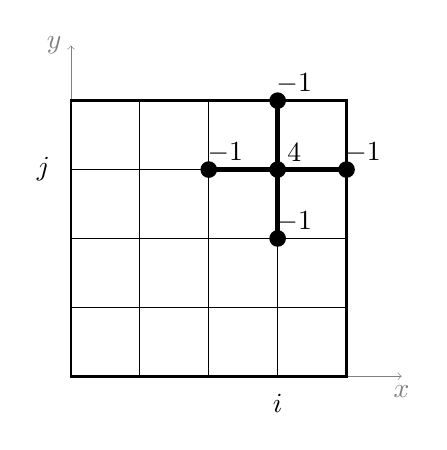
\begin{tikzpicture}[scale=3.5]
  \draw[->,gray,very thin] (0.0,0.0) -- (1.2,0.0) node[below] {$x$};
  \draw[->,gray,very thin] (0.0,0.0) -- (0.0,1.2) node[left] {$y$};
  \draw[line width=1.0pt] (0.0,0.0) -- (0.0,1.0) -- (1.0,1.0) -- (1.0,0.0) -- cycle;
  \node at (0.75,-0.1) {$i$};
  \node at (-0.1,0.75) {$j$};
  \filldraw (0.50,0.75) circle (0.8pt);
  \filldraw (0.75,0.75) circle (0.8pt);
  \filldraw (1.00,0.75) circle (0.8pt);
  \filldraw (0.75,0.5) circle (0.8pt);
  \filldraw (0.75,1.0) circle (0.8pt);
  \pgfmathsetmacro\dd{0.06}
  \draw (0.75+\dd,0.75+\dd) node{$4$};
  \draw (0.5+\dd,0.75+\dd)  node{$-1$};
  \draw (0.75+\dd,0.5+\dd)  node{$-1$};
  \draw (1.0+\dd,0.75+\dd)  node{$-1$};
  \draw (0.75+\dd,1.0+\dd)  node{$-1$};
  \draw[line width=2.0pt] (0.50,0.75) -- (1.00,0.75);
  \draw[line width=2.0pt] (0.75,0.5)  -- (0.75,1.00);
  \draw[xstep=0.25,ystep=0.25,black,thin] (0.0,0.0) grid (1.0,1.0);
\end{tikzpicture}
\caption{For a grid with $h_x=h_y$, the coefficients on the left side of \eqref{poissonsquareFD} are the well-known ``$4$'' and ``$-1$'' for the stencil of the Laplacian.}
\label{fig:equalstarstencil}
\end{marginfigure}

Our second observation is that the FD equations can be re-interpreted to give a \emph{symmetric} matrix $A$.  For example, in the $i=1$ case of \eqref{poissonsquareFD}, i.e.~at a grid point adjacent to the left-hand boundary of the square, the boundary location value $U_{0,j}$ appears in the equation.  The matrix in the linear system will be symmetric if we systematically ``move'' such values to the right-hand side as known.  That is, we force off-diagonal matrix entries to be zero in columns corresponding to known boundary values.  Converting to a symmetric system opens up a larger range of linear algebra methods for solving the system efficiently, including conjugate gradients (\texttt{-ksp\_type cg}) and Cholesky preconditioners (\texttt{-pc\_type cholesky} or \texttt{-pc\_type icc}).

With these two modifications we can redo the last example.

\medskip\noindent\hrulefill
\begin{example} For the same $M=4$ and $N=3$ case shown in Figure \ref{fig:unitsquaregridordering}, equations \eqref{poissonsquareFDbcs} and \eqref{poissonsquareFD} yield the linear system
\begin{equation*}
\begin{bmatrix}
1 &  &  &  &  &  &  &  &  &  &  &  \\
  & 1&  &  &  &  &  &  &  &  &  &  \\
  &  & 1&  &  &  &  &  &  &  &  &  \\
  &  &  & 1&  &  &  &  &  &  &  &  \\
  &  &  &  & 1&  &  &  &  &  &  &  \\
  &  &  &  &  & \alpha& \beta&  &  &  &  &  \\
  &  &  &  &  & \beta& \alpha&  &  &  &  &  \\
  &  &  &  &  &  &  & 1&  &  &  &  \\
  &  &  &  &  &  &  &  & 1&  &  &  \\
  &  &  &  &  &  &  &  &  & 1&  &  \\
  &  &  &  &  &  &  &  &  &  & 1&  \\
  &  &  &  &  &  &  &  &  &  &  & 1
\end{bmatrix}
\begin{bmatrix}
U_{0,0} \\
U_{1,0} \\
U_{2,0} \\
U_{3,0} \\
U_{0,1} \\
U_{1,1} \\
U_{2,1} \\
U_{3,1} \\
U_{0,2} \\
U_{1,2} \\
U_{2,2} \\
U_{3,2}
\end{bmatrix}
=
\begin{bmatrix}
0 \\
0 \\
0 \\
0 \\
0 \\
(1/6) f_{1,1} \\
(1/6) f_{2,1} \\
0 \\
0 \\
0 \\
0 \\
0
\end{bmatrix}
\end{equation*}
where $\alpha = 2 (h_y/h_x) + 2 (h_x/h_y) = 13/3$ and $\beta = - h_y/h_x = - 3/2$.  The matrix is symmetric, positive definite, and better-scaled than before with $\kappa(A)=5.83$.
\end{example}
\noindent\hrulefill

\medskip
\section{Code for matrix assembly}

We now show in Figure \ref{code:structuredpoisson} the code that assembles ``$A$'' in linear system \eqref{poissonlinearsystem}.  For clarity and code reuse we have isolated this method in a separate file.  Arguments to \texttt{formdirichletlaplacian()} include the \pDM itself, grid spacings \texttt{hx,hy}, the value to put on the diagonal for Dirichlet boundary conditions, and the returned (i.e.~modified) \pMat \texttt{A}.

\cinputpart{structuredpoisson.c}{Fill matrix entries using \texttt{MatSetValuesStencil}.  (From now on we strip ``\texttt{ierr=}'' and ``\texttt{CHKERRQ(ierr)}'' from the displayed code, but it is still present in the source.)}{I}{//CREATEMATRIX}{//ENDCREATEMATRIX}{code:structuredpoisson}

The argument ``\texttt{DMDALocalInfo info}'' needs special description.  As shown in Figure \ref{fig:localpartofgrid}, \texttt{info} is a C structure which stores both global grid size and the extent of the locally-owned subgrid.  The global size is in members \texttt{info.mx,info.my}.  The local process owns a \texttt{info.xm} by \texttt{info.ym} rectangular subgrid, with a range of indices
\begin{align*}
&\text{\texttt{info.xs}} \le i \le \text{\texttt{info.xs}} +\text{\texttt{info.xm}}-1, \\
&\text{\texttt{info.ys}} \le j \le \text{\texttt{info.ys}} +\text{\texttt{info.ym}}-1.
\end{align*}
in two dimensions.  For example, in Figure \ref{fig:unitsquaregridparallel} the rank $0$ and $2$ processes have \text{\texttt{info.xs}} $=0$ and \text{\texttt{info.xm}} $=3$ while the rank $1$ and $3$ processes have \text{\texttt{info.xs}} $=3$ and \text{\texttt{info.xm}} $=2$.  The $y$ ranges are similar.

\begin{figure}
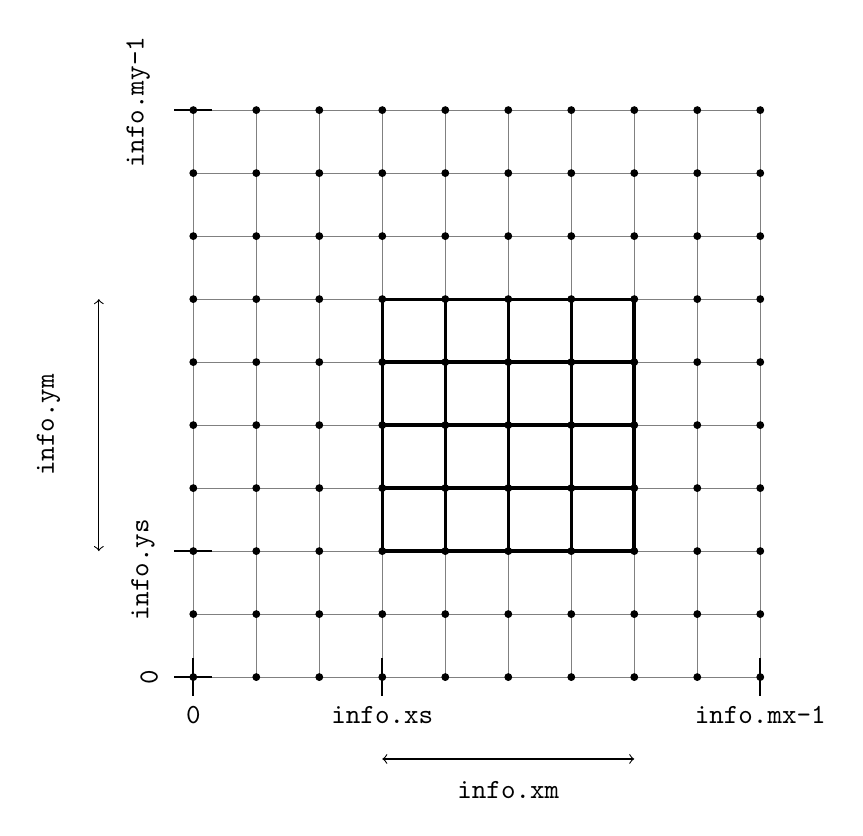
\begin{tikzpicture}[scale=8]
  % global grid, local grid, nodes
  \draw[xstep=0.1,ystep=0.1,gray,very thin] (0.0,0.0) grid (0.9,0.9);
  \draw[xstep=0.1,ystep=0.1,black,very thick] (0.3,0.2) grid (0.7,0.6);
  \foreach \y in {0,...,9}
    \foreach \x in {0,...,9} {
      \filldraw (\x * 0.1,\y * 0.1) circle (0.15pt);
    }
  % ticks on x-axis at 0, xs, mx
  \draw[black,thick] (0,-0.03)   -- (0,+0.03);
  \draw[black,thick] (0.3,-0.03) -- (0.3,+0.03);
  \draw[black,thick] (0.9,-0.03) -- (0.9,+0.03);
  \node at (0,-0.06) {\texttt{0}};
  \node at (0.3,-0.06) {\texttt{info.xs}};
  \node at (0.9,-0.06) {\texttt{info.mx-1}};
  % ticks on y-axis at 0, ys, my
  \draw[black,thick] (-0.03,0)   -- (+0.03,0);
  \draw[black,thick] (-0.03,0.2) -- (+0.03,0.2);
  \draw[black,thick] (-0.03,0.9) -- (+0.03,0.9);
  \node[rotate around={90:(0,0)}] at (-0.07,0) {\texttt{0}};
  \node[rotate around={90:(-0.2,0.2)}] at (-0.08,0.12) {\texttt{info.ys}};
  \node[rotate around={90:(0.0,0.9)}] at (-0.20,0.8) {\texttt{info.my-1}};
  % xm, ym along sides of local patch
  \draw[<->,] (0.3,-0.13) -- (0.7,-0.13);
  \node at (0.5,-0.18) {\texttt{info.xm}};
  \draw[<->,] (-0.15,0.2) -- (-0.15,0.6);
  \node[rotate around={90:(0.3-0.3,0.4)}] at (-0.28,0.35) {\texttt{info.ym}};
\end{tikzpicture}
\caption{A \texttt{DMDALocalInfo} struct describes the indices for a local process' part of a 2D grid, plus the global grid size, using six integers.}
\label{fig:localpartofgrid}
\end{figure}

The index ranges from \texttt{info} are used in the \texttt{for} loops which re-appear every time we do operations on a structured 2D grid:
\begin{code}
for (j=info.ys; j<info.ys+info.ym; j++) {
  for (i=info.xs; i<info.xs+info.xm; i++) {
    DO SOMETHING AT GRID POINT (i,j)
  }
}
\end{code}

Still considering the code in Figure \ref{code:structuredpoisson}, the \pMat object $A$ assembled by \texttt{formdirichletlaplacian()}  has ranges of rows owned by each process, the standard parallel layout \texttt{MATMPIAIJ} of \pMat objects in \PETSc (Chapter \ref{chap:getstarted}).  However, because we work with the locally-owned subgrid using $(i,j)$ indices, we can often forget the actual layout of a \pMat.  We get to just focus on the part of the grid owned by the process, as in Figures \ref{fig:unitsquaregridparallel}--\ref{fig:unitsquaregrideight}, instead of worrying about the matrix itself.

In particular, local indices $(i,j)$ can be used when inserting entries into \pMat \texttt{A}, which is really a dynamical data structure for matrix assembly.  Thus in Figure \ref{code:structuredpoisson} we see one use of \texttt{MatSetValuesStencil()} for each locally-owned grid point.  For a generic interior point this command inserts five coefficients into the matrix.  The key data structure is of type \texttt{MatStencil}, an apparently-trivial struct
\begin{code}
typedef struct {
  PetscInt k,j,i,c;
} MatStencil;
\end{code}
In our 2D case, with a single degree of freedom at each node,\sidenote{The Poisson equation \eqref{poissonsquare} is a scalar PDE so the unknown at each grid point is the scalar $U_{i,j}$.  A system of equations like Navier-Stokes would have \texttt{dof}$>1$ when we call \texttt{DMDACreateXd()}, and the ``\texttt{c}'' member of \texttt{MatStencil} would get used.} we only use the \texttt{i} and \texttt{j} members of \texttt{MatStencil}.  From \eqref{poissonsquareFD}, the actual matrix entries are $a_{i,i} = 2\left(h_y/h_x + h_x/h_y\right)$ on the diagonal, and $a_{i,j} = -h_y/h_x$ or $a_{i,j} = -h_x/h_y$ for off-diagonals.  We only insert nonzero off-diagonals in the matrix if the column corresponds to a non-boundary location.  After completing all the \texttt{MatSetValuesStencil()} insertion commands we call \texttt{MatAssemblyBegin/End()} just as we did in Chapter \ref{chap:getstarted}.


\section{A particular problem, an exact solution}

At this point we need to set up a particular Poisson problem so our first example code can solve it.  To do this we again\sidenote{For the code \texttt{c1tri.c} in Chapter 1 we did something similar, i.e.~the choice of exact solution $\bu$ before computing $\bb=A\bu$ by matrix multiplication.} \emph{choose} an exact solution, taking care that it satisfies homogeneous Dirichlet boundary conditions ($u=0$ along $\partial \mathcal{S}$):
\begin{equation}
u(x,y) = (x^2 - x^4) (y^4 - y^2). \label{exactsolution}
\end{equation}
Then we merely differentiate to get $f = -\grad^2 u$.  Thus \eqref{exactsolution} solves \eqref{poissonsquare} with right side
\begin{equation}
f(x,y) = 2 (1 - 6 x^2) y^2 (1 - y^2) + 2 (1 - 6 y^2) x^2 (1 - x^2).\label{manufacturedf}
\end{equation}
From now on we will refer to $u$ in \eqref{exactsolution} as ``$u_{ex}$'', the exact solution.  This same problem and solution appears in Chapter 4 of \citep{Briggsetal2000}, so these formulas are not original. % page 64

Observe that the truncation error term $O(h^2)$ in equation \eqref{secondderivativeFD} has a coefficient proportional to fourth derivatives \citep{MortonMayers} so our FD method will not be exact on this problem because $u_{ex}$ has nonzero fourth derivatives.  This is \emph{good}.  We would not use the simpler form $u(x,y)=(x-x^2)(y-y^2)$, for example, to test convergence rate of the code because the decay of numerical error with refining grids is not at all generic.

Because we want to reuse this part also,\sidenote{See Chapter \ref{chap:multigrid}.} we put the code that computes formulas \eqref{exactsolution} and \eqref{manufacturedf} in source file \texttt{structuredpoisson.c}.  Figure \ref{code:poissonexactrhs} shows how \eqref{exactsolution} is implemented as \texttt{formExact()} and how \eqref{manufacturedf} is implemented as \texttt{formRHS()}.

\vfill
\newpage
\cinputpart{structuredpoisson.c}{Methods which assemble \pVec \texttt{uexact} for the exact solution and \pVec \texttt{b} for the right-hand side of equation \eqref{poissonsquareFD}.}{II}{//FORMEXACTRHS}{//ENDFORMEXACTRHS}{code:poissonexactrhs}

The computations in Figure \ref{code:poissonexactrhs} use only local grid coordinates $(i,j)$, with loops over index ranges as shown in Figure \ref{fig:localpartofgrid}.  \PETSc pointer arithmetic (i.e.~tricks) allows us to index the C arrays we get from \texttt{DMDAVecGetArray()} using $(i,j)$.  When we are done with computing \pVecs we restore the C arrays by calling \texttt{DMDAVecRestoreArray()}, and we explicitly ask for the \pVec objects to be assembled by calling \texttt{VecAssemblyBegin/End()}, just as in Chapter \ref{chap:getstarted}.


\vfill
\newpage
\section{Solving the PDE}

The code \texttt{c2poisson.c} uses our finite difference method \eqref{poissonsquareFD} to solve the Poisson problem with $f$ from \eqref{manufacturedf}.  Figure \ref{code:ctwopoissoncreate} shows how \texttt{c2poisson.c} creates the various parallel objects needed to solve the Poisson problem, namely one \pDM, one \pMat, and three \pVecs.  A \pDM object can compute matrix and vector sizes from the grid dimensions, so we call \texttt{DMCreateMatrix()} and \texttt{DMCreateGlobalVector()} to create \pMat and \pVec objects, respectively.  Then we call methods from \texttt{structuredpoisson.c}, as above, to assemble the matrix and vectors.

\cinputpart{c2poisson.c}{Set up \pDM, \pMat, and \pVec objects, and assemble the linear system.}{I}{//CREATE}{//ENDCREATE}{code:ctwopoissoncreate}

\vfill
\newpage
\PETSc describes the linear system ``$A\bu=\bb$'' by one \pMat \texttt{A} and two \pVecs (\texttt{u} and \texttt{b}), but, as in Chapter \ref{chap:getstarted}, the method for solving the linear system is a Krylov space method solver object of type \pKSP.  The part of \texttt{c2poisson.c} that creates and uses this object is in Figure \ref{code:ctwopoissonsolve}.  After calling \texttt{KSPSolve()} we compute the numerical error with \texttt{VecAXPY()} and \texttt{VecNorm()}, this time computing the error $\|u-u_{ex}\|_\infty$.  Finally we print the error and clean up.

\cinputpart{c2poisson.c}{Solve using \pKSP, and report on solution.}{II}{//SOLVE}{//ENDSOLVE}{code:ctwopoissonsolve}

To finish showing the code, in Figure \ref{code:ctwopoissonsolve} we create the \pKSP object and tell it about \texttt{A} through a call to \texttt{KSPSetOperators()}.  Inside a \pKSP there are two ways \texttt{A} is used, namely as the system matrix and as a possible preconditioner---more on this later---which explains why \texttt{A} appears twice when calling \texttt{KSPSetOperators()}.  We also call \texttt{KSPSetFromOptions()} so that we can change the \pKSP type at runtime (illustrated below).  Solving the system means calling \texttt{KSPSolve()}.  Then we report on the solution by computing the numerical error by the norm $\|u-u_{ex}\|_\infty$.  Then we wrap up by destroying objects and calling \texttt{PetscFinalize()}.


\section{Runtime control}

As a first run do:
\begin{cline}
$ make c2poisson
$ ./c2poisson
\end{cline}
to get output
\begin{cline}
on 10 x 10 grid:  error |u-uexact|_inf = 0.000621778
\end{cline}
We see the default $10\times 10$ grid chosen in our call to \texttt{DMDACreate2d()}. There were seven iterations of the KSP method and a final residual norm and numerical error.

At this point we want to know:\begin{itemize}
\item is our numerical method correctly implemented? (\emph{convergence})
\item how to get high performance? (\emph{efficiency})
\item how to see inside \PETSc so we know what is going on? (\emph{exposure})
\end{itemize}
In \PETSc these choices of solver and parameters are controllable and exposable at runtime, once we have adequately-described the problem to \PETSc.  We can both put-off questions of convergence, scaling, and exposure until runtime, and we can make control choices empirically, i.e.~based on actual performance.  Runtime control is a topic that we will return to frequently, starting now with measuring convergence of \texttt{c2poisson.c}.


\section{Convergence}

By ``showing convergence'' we mean that we demonstrate that errors made by our numerical solver decrease in the expected way, as we refine the grid so that the finite differences are better approximations of the corresponding derivatives.  Furthermore we want to show that the rate at which the error decreases matches what we expect in theory.

There are two ways to specify a finer grid in a code like \texttt{c2poisson.c}, both of which address the \pDM object through options.  One is to specify the grid directly:
\begin{cline}
$ ./c2poisson -da_grid_x 100 -da_grid_y 100
on 100 x 100 grid:  error |u-uexact|_inf = 5.76054e-06
\end{cline}
%$
The other is to instruct the \pDM to refine the grid by factors of two.  More precisely, the number of \emph{subintervals} is increased by a factor of two.  For example, this call replaces our default grid of 9 by 9 subintervals (i.e.~10 by 10 grid \emph{points}) by 18 subintervals in each direction (i.e.~19 grid points):
\begin{cline}
$ ./c2poisson -da_refine 1
on 19 x 19 grid:  error |u-uexact|_inf = 0.000155374
\end{cline}
%$

We check convergence by generating error data.  Here is a loop using the Bash shell:
\begin{cline}
$ for K in 0 1 2 3 4 5 6; do ./c2poisson -da_refine $K; done
on 10 x 10 grid:  error |u-uexact|_inf = 0.000621778
on 19 x 19 grid:  error |u-uexact|_inf = 0.000155374
on 37 x 37 grid:  error |u-uexact|_inf = 3.87982e-05
on 73 x 73 grid:  error |u-uexact|_inf = 1.05331e-05
on 145 x 145 grid:  error |u-uexact|_inf = 3.17389e-06
on 289 x 289 grid:  error |u-uexact|_inf = 1.60786e-06
on 577 x 577 grid:  error |u-uexact|_inf = 1.22251e-06
\end{cline}
%$
The data is shown in Figure \ref{fig:c2poisson-conv} as the squares.  For the coarser grids (e.g.~$N+1=10,19,37,73$ grid points), a refinement by a factor of two gives a reduction in error by a factor of about four, as expected because our FD method is $O(h^2)$ \citep{MortonMayers}.  Unfortunately the error seems to have stopped falling for the finer grids ($N+1=145,289,577$), at a level around $\|u-u_{ex}\|_\infty \approx 10^{-6}$.

\begin{figure}
\bigskip
\includegraphics[width=0.9\textwidth]{c2poisson-conv}
\caption{To show convergence we refine the \pDM grid by factors of two.  With the default \pKSP relative tolerance the error seems to level out (squares).  With a stronger tolerance for solving the linear system (\texttt{-ksp\_rtol 1.0e-12}) the errors continue to fall (circles) at the expected rate (dotted line).}
\label{fig:c2poisson-conv}
\end{figure}

Is the reduce apparent rate of convergence a sign of an implementation error.  In fact not, because simply asking for the \pKSP object to solve the linear system better is effective.  On a particular grid we can see the difference using option \texttt{-ksp\_monitor} to watch the residuals and setting a stronger value for the \pKSP relative tolerance for residual norm size (\texttt{-ksp\_rtol}):
\begin{cline}
$ ./c2poisson -ksp_monitor
  0 KSP Residual norm 1.007660904704e-01 
  1 KSP Residual norm 2.917206076870e-02 
  2 KSP Residual norm 1.153582666339e-02 
... 
  6 KSP Residual norm 6.995040432502e-06 
  7 KSP Residual norm 8.593881990968e-07 
on 10 x 10 grid:  error |u-uexact|_inf = 0.000621778
$ ./c2poisson -ksp_monitor -ksp_rtol 1.0e-12
  0 KSP Residual norm 1.007660904704e-01 
  1 KSP Residual norm 2.917206076870e-02 
  2 KSP Residual norm 1.153582666339e-02 
...
 13 KSP Residual norm 4.240214646869e-13 
 14 KSP Residual norm 3.105665682224e-14 
on 10 x 10 grid:  error |u-uexact|_inf = 0.000621527
\end{cline}
On this coarse grid the numerical error is nearly the same, but on finer grids the fact that the linear system is solved more exactly will bring the numerical solution closer to the exact one.  However, the \pKSP takes twice as many iterations to achieve the desired residual norm reduction.

In fact, rerunning the Bash loop with the stronger tolerance yields excellent evidence of convergence at the expected rate:
\begin{cline}
$ for K in 0 1 2 3 4 5 6; do ./c2poisson -da_refine $K -ksp_rtol 1.0e-12; done
on 10 x 10 grid:  error |u-uexact|_inf = 0.000621527
on 19 x 19 grid:  error |u-uexact|_inf = 0.000155312
on 37 x 37 grid:  error |u-uexact|_inf = 3.8823e-05
on 73 x 73 grid:  error |u-uexact|_inf = 9.71122e-06
on 145 x 145 grid:  error |u-uexact|_inf = 2.42806e-06
on 289 x 289 grid:  error |u-uexact|_inf = 6.07041e-07
on 577 x 577 grid:  error |u-uexact|_inf = 1.51761e-07
\end{cline}
%$
This is plotted as the circles in Figure \ref{fig:c2poisson-conv}.  The linear-fit rate of this logarithmic error data is $O(h^{1.9999})$.  Our implementation is correct in this sense.


\section{Efficiency, and exposing \PETSc's solvers}

On the other hand, the finer grid calculations above are slow.  How about if we re-run in parallel?  On a typical four-core laptop\sidenote{Circa 2013 manufacture, with an Intel i7 processor at 2.7GHz.} we get:
\begin{cline}
$ time ./c2poisson -da_refine 5 -ksp_rtol 1.0e-12
on 289 x 289 grid:  error |u-uexact|_inf = 6.07041e-07
real 31.53
user 31.40
sys 0.09
$ time mpiexec -n 4 ./c2poisson -da_refine 5 -ksp_rtol 1.0e-12
on 289 x 289 grid:  error |u-uexact|_inf = 6.07041e-07
real 12.63
user 45.41
sys 0.38
\end{cline}
It is nice to see a speedup, though only by a factor of $31.5/12.6 = 2.5$ on this fixed-size problem, which is disappointing given the putative four-times increase in processing power.

These first performance results probably raise more questions than they answer.  In particular,
\renewcommand{\labelenumi}{\roman{enumi})}
\begin{enumerate}
\item are we effectively using \PETSc options at runtime?
\item what is going on inside the \PETSc solver(s)?
\item is this the parallel scaling we expect?
\item was our method actually efficient?
\end{enumerate}
While we will focus on performance and scaling in Chapter \ref{chap:scaling}, we can get started on these questions.

Regarding i), even knowing what are possible runtime options is nontrivial in \PETSc because there are so many options.  But the answer is simple: pipe the output from option \texttt{-help} into a pager like \texttt{more} or \texttt{less}, like this
\begin{cline}
$ ./c2poisson -help | less
\end{cline}
%$
This gives a view of the options available \emph{for} \texttt{c2poisson}, so that, for instance, the many options for nonlinear solvers are \emph{not} included in \texttt{-help} output because we have not used \pSNES; we'll use such tools in Chapter \ref{chap:nonlinear}.  This \texttt{-help} output also gives default values for parameters; for example we see that the default for \texttt{-ksp\_rtol} is \texttt{1e-05}, which explains why convergence ``leveled out'' on fine grids.

Alternatively, one might want to know what are options for controlling particular objects inside \texttt{c2poisson}.  For example, this command shows runtime options which control the \pKSP object:
\begin{cline}
$ ./c2poisson -help | grep ksp_
\end{cline}
%$
If the list is too long, pipe it into the pager:
\begin{cline}
$ ./c2poisson -help | grep ksp_ | less
\end{cline}
%$

Regarding ii), recall that we used \texttt{-dm\_view} to show properties of the \pDM object in \texttt{c2poisson}.  We should do the same for the \pKSP object:
\begin{cline}
$ ./c2poisson -ksp_view
KSP Object: 1 MPI processes
  type: gmres
    GMRES: restart=30, using Classical (unmodified) Gram-Schmidt Orthogonaliz...
    GMRES: happy breakdown tolerance 1e-30
  maximum iterations=10000, initial guess is zero
  tolerances:  relative=1e-05, absolute=1e-50, divergence=10000
  left preconditioning
  using PRECONDITIONED norm type for convergence test
PC Object: 1 MPI processes
  type: ilu
    ILU: out-of-place factorization
    ...
  linear system matrix = precond matrix:
  Mat Object:  (a_)   1 MPI processes
    type: seqaij
    rows=100, cols=100
    total: nonzeros=460, allocated nonzeros=460
    ...
on 10 x 10 grid:  iterations 7, residual norm = 8.59388e-07,
                  error |u-uexact|_inf = 0.000621778
\end{cline}
%$
We have suppressed some of the output, but this shows the default FIXME

FIXME but wait, $A$ was symmetric; show
\begin{cline}
$ ./c2poisson -ksp_type cg
\end{cline}
%$

FIXME:  In parallel
\begin{cline}
$ mpiexec -n 4 ./c2poisson -ksp_view
...
\end{cline}
%$



\section{Time-dependent heat equation}

FIXME: we WON'T do explicit, but it would look like ...

FIXME: use TS for backward-euler




\section{Exercises}

\renewcommand{\labelenumi}{\arabic{chapter}.\arabic{enumi}\quad}
\begin{enumerate}
\item FIXME modify \texttt{c2poisson.c} to do non-homogeneous Dirichlet
\end{enumerate}